\documentclass[english]{article}
\usepackage[table]{xcolor}
\usepackage{amsmath}
\usepackage{amssymb}
\usepackage[utf8]{inputenc}
\usepackage{tikz}
\usetikzlibrary{positioning} 
\usetikzlibrary{matrix}
\usetikzlibrary{patterns}
\usetikzlibrary{fit}
\usetikzlibrary{shapes, arrows.meta}

\begin{document}

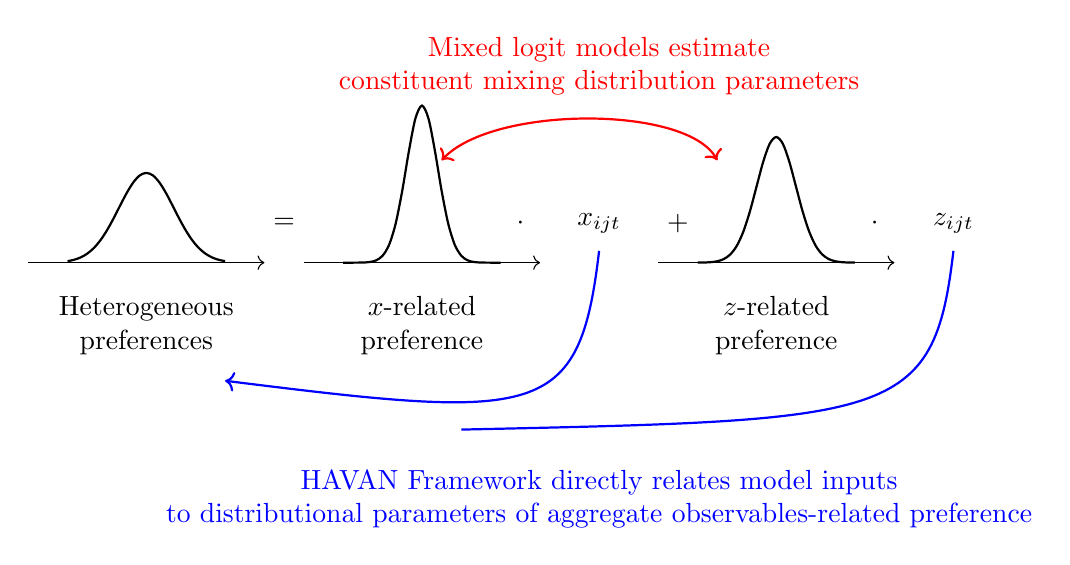
\begin{tikzpicture}
    \draw[white](0,0)--(0,0);
    \begin{scope}[shift={(0,0)}]
        \draw[->] (-1.5,0) -- (1.5,0) node[right] {};
        
        % Adjusted standard deviation
        \def\stddev{0.35}
        
        % Normal distribution curve
        \draw[smooth, thick, domain=-1:1] plot (\x, {exp(-\x*\x/(2*\stddev*\stddev))/(sqrt(2*pi)*\stddev)});
    \end{scope}

    \node[black] at (1.75,0.5) {=};

    \begin{scope}[shift={(3.5,0)}]
        \draw[->] (-1.5,0) -- (1.5,0) node[right] {};
        
        % Adjusted standard deviation
        \def\stddev{0.2}
        
        % Normal distribution curve
        \draw[smooth, thick, domain=-1:1] plot (\x, {exp(-\x*\x/(2*\stddev*\stddev))/(sqrt(2*pi)*\stddev)});
    \end{scope}

    \node[black] at (4.75,0.5) {$\cdot$};
    \node[black] at (5.75,0.5) {$x_{ijt}$};
    \node[black] at (6.75,0.5) {+};

    \begin{scope}[shift={(8,0)}]
        \draw[->] (-1.5,0) -- (1.5,0) node[right] {};
        
        % Adjusted standard deviation
        \def\stddev{0.25}
        
        % Normal distribution curve
        \draw[smooth, thick, domain=-1:1] plot (\x, {exp(-\x*\x/(2*\stddev*\stddev))/(sqrt(2*pi)*\stddev)});
    \end{scope}

    \node[black] at (9.25,0.5) {$\cdot$};
    \node[black] at (10.25,0.5) {$z_{ijt}$};
    
    \node[black, align=center] at (0,-0.8) {Heterogeneous\\preferences};
    \node[black, align=center] at (3.5,-0.8) {$x$-related\\preference};
    \node[black, align=center] at (8,-0.8) {$z$-related\\preference};

    % Red curved arrow and text
    \draw[red, <->, thick] (3.75, 1.3) .. controls (4.4,2) and (6.875,2) .. (7.25, 1.3);
    \node[red, align=center] at (5.75,2.5) {Mixed logit models estimate\\constituent mixing distribution parameters};
    
    % Blue arrows and text
    \draw[blue, ->, thick] (5.75, 0.15) .. controls (5.5,-2) and (5,-2) .. (1, -1.5);
    \draw[blue, -, thick] (10.25, 0.15) .. controls (10,-2) and (9.5,-2) .. (4, -2.12);
    \node[blue, align=center] at (5.75,-3) {HAVAN Framework directly relates model inputs\\to distributional parameters of aggregate observables-related preference};
\end{tikzpicture}

\end{document}